\documentclass[12px]{report}

%
%   Packages
%
\usepackage[a4paper,top=2cm,bottom=2cm,left=2cm,right=2cm]{geometry}
\usepackage{graphicx}
\usepackage[sorting=none]{biblatex}
\usepackage[acronym]{glossaries}
\usepackage[english]{babel}
\usepackage{csquotes}
\usepackage{setspace}
\usepackage{makecell}

%
%   Line spacing
%
\setstretch{1.5}


%
%   Utilities and costants
%
\def\blankpage{
    \clearpage
    \thispagestyle{empty}
    \addtocounter{page}{-1}
    \null
    \clearpage
}

%
%   Acronyms
%
\newacronym{ms}{MS}{\textit{Mobile system}}
\newacronym{dos}{DOS}{\textit{Denial Of Service}}
\newacronym{iot}{IOT}{\textit{Internet Of Things}}
\newacronym{ran}{RAN}{\textit{Radio Access Network}}
\newacronym{ue}{UE}{\textit{User Equipment}}
\newacronym{bs}{BS}{\textit{Base Station}}
\newacronym{sim}{SIM}{\textit{Subscriber Identity Module}}
\newacronym{mtso}{MTSO}{\textit{Mobile Telephone Switching Office}}
\newacronym{fdma}{FDMA}{\textit{Frequency Division Multiple access}}
\newacronym{gsm}{GSM}{\textit{Global System for Mobile Communications}}
\newacronym{sms}{SMS}{\textit{Short Message Service}}
\newacronym{bss}{BSS}{\textit{Base Station Subsystem}}
\newacronym{nss}{NSS}{\textit{Network Switching Subsystem}}
\newacronym{msc}{MSC}{\textit{Mobile  Switching  Center}}
\newacronym{ptsn}{PTSN}{\textit{Public switched telephone network}}
\newacronym{hlr}{HLR}{\textit{Home Location Register}}
\newacronym{vlr}{VLR}{\textit{Visitor Location Register}}
\newacronym{eir}{EIR}{\textit{Equipment Identity Register}}
\newacronym{auc}{AuC}{\textit{Authentication Center}}
\newacronym{gprs}{GPRS}{\textit{General Packet Radio Service}}
\newacronym{sgsn}{SGSN}{\textit{Serving GPRS Support Node}}
\newacronym{wcdma}{W-CDMA}{\textit{Wideband Code Division Multiple Access}}
\newacronym{umts}{UMTS}{\textit{Universal Mobile Telecommunications System}}
\newacronym{ggsn}{GGSN}{\textit{Gateway GPRS Support Node}}
\newacronym{ip}{IP}{\textit{Internet Protocol}}
\newacronym{hss}{HSS}{\textit{Home Subscriber Server}}
\newacronym{mme}{MME}{\textit{Mobility Management Entity}}
\newacronym{sgw}{S-GW}{\textit{Serving - Gateway}}
\newacronym{lte}{LTE}{\textit{Long Term Evolution}}
\newacronym{pgw}{P-GW}{\textit{Packet data network - Gateway}}
\newacronym{pcrf}{PCRF}{\textit{Policy Control and Charging Rules Function}}
\newacronym{sba}{SBA}{\textit{Service Base Architecture}}
\newacronym{sdn}{SDN}{\textit{Software Defined Network}}
\newacronym{ddos}{DDOS}{\textit{Distributed Denial Of Service}}
\newacronym{aka}{AKA}{\textit{Authentication and Key Agreement}}
\newacronym{imsi}{IMSI}{\textit{International Mobile Subscriber Identity}}
\newacronym{imei}{IMEI}{\textit{International Mobile Equipment Identity}}
\newacronym{tmsi}{TMSI}{\textit{Temporary Mobile Subscriber Identity}}
\newacronym{sres}{SRES}{\textit{Signed Response}}
\newacronym{suci}{SUCI}{\textit{Subscription Concealed Identifier}}
\newacronym{ik}{IK}{\textit{Integrity Key}}
\newacronym{snn}{SNN}{\textit{Serving Network Name}}
\newacronym{tps}{TPS}{\textit{Transation Per Second}}
\newacronym{nfv}{NFV}{\textit{Network Functions Virtualization}}
\newacronym{mitm}{MITM}{\textit{Man In The Middle}}
\newacronym{ecies}{ECIES}{\textit{Elliptic Curve Integrated Encryption Scheme}}
\newacronym{supi}{SUPI}{\textit{Subscription Permanent Identifier}}
\newacronym{smf}{SMF}{\textit{Session Management Function}}
\newacronym{pcf}{PCF}{\textit{Policy Control Function}}
\newacronym{udm}{UDM}{\textit{Unified Data Management}}
\newacronym{ausf}{AUSF}{\textit{Authentication Server Function}}
\newacronym{sdsf}{SDSF}{\textit{Structured Data Storage Network Function}}
\newacronym{udsf}{UDSF}{\textit{Unstructured Data Storage Network Function}}
\newacronym{aria}{ARIA}{\textit{Air Pollutants Monitoring Using UAVs}}
\newacronym{cots}{COTS}{\textit{Commercial off-the-shelf}}
\newacronym{uavs}{UAVs}{\textit{Unmanned Aerial Vehicles}}
\newacronym{wsn}{WSN}{\textit{Wireless Sensor Network}}
\newacronym{epa}{EPA}{Environmnetal Protection Agengy}
\newacronym{nef}{NEF}{\textit{Network Exposure Function}}
\newacronym{nrf}{NRF}{\textit{Network Repository Function}}
\newacronym{nssf}{NSSF}{\textit{Network Slicing Selector Function}}
\newacronym{upf}{UPF}{\textit{User Plane Function}}
\newacronym{amf}{AMF}{\textit{Access and Mobility Management Function}}
\newacronym{seaf}{SEAF}{\textit{Security Anchor Function}}
\newacronym{guti}{GUTI}{\textit{Globally Unique Temporary Identifier}}
\newacronym{fach}{FACH}{\textit{Forward Access Channel}}
\newacronym{autn}{AUTN}{\textit{Authentication Token}}
\makenoidxglossaries

%
%   References
%
\addbibresource{formats/references.bib}

%
%   Document
%
\begin{document}
    \begin{titlepage}
  \begin{center}
    
\includegraphics[width=0.3\textwidth]{images/unipd.png}
    \hfill
    
\includegraphics[width=0.3\textwidth]{images/dei.png}
  \end{center}
  \begin{center}
    \vspace{3cm}
    \large
    \MakeUppercase{
      \textbf{
        Dipartimento di ingegneria dell'informazione\\
        \vspace{0.5cm}
        Corso di laurea in Ingegneria Informatica\\
      }
    }
    \vspace{4cm}
    \MakeUppercase{
      \textbf{
        Sviluppo del software di acquisizione ed elaborazione delle misure dell'inquinamento dell'aria di droni progetto A.R.I.A.\\
      }
    }
    \vspace{4cm}
    \begin{flushleft}
      \textbf{
        Relatore: Prof. Carlo Bettanini Fecia di Cossato\\
      }
    \end{flushleft}
    \vspace{1cm}
    \begin{flushright}
      \textbf{
        Laureando: Giacomo Favaron\\
      }
    \end{flushright}
    \vspace{2.5cm}
    \MakeUppercase{
      \textbf{
        Anno accademico: 2020-2021\\
      }
    }
    \vspace{0.5cm}
    \textbf{
      Data di laurea: 15/11/2021
    }
  \end{center}
\end{titlepage}
    %\blankpage
    \begin{abstract}
In the recent years, awareness of the issue of Environmental Pollution has increased, and research shows that not enough has been done, until now, to reduce pollution. In this domain, the monitoring of air quality is fundamental to provide data which can be used to most effectively guide our efforts to reduce air pollution. At this time the monitoring of air quality is usually performed via stationary ground-mounted air pollution stations. However, research(??) has shown that air pollution can vary greatly at different heights, for this reason the \gls{aria} project is aiming to develop a system to measure vertical gradients of air pollutants using vertical swarms of drones. The \gls{aria} project solution is a low-cost monitoring system based on \gls{cots} sensors and on multiple cheap drone platforms. The system is equipped with $PM_2.5$ and $PM_10$ sensors to monitor the particulate concentration and several other gas sensors (such as $NO$, $NO_2$, $CO$, etc.) and the use of \gls{uavs} allows to build a 3D map of pollutants in a specific area. This could prove very useful around buildings in urban areas and possibile polluting plants in industrial areas. In this thesis are presented the system platform, the software implementation and a test flight.
\end{abstract}
    \clearpage
    \tableofcontents{}
    \clearpage
    \listoffigures
    \clearpage
    \printnoidxglossary[type=acronym, title={List of abbreviations}, style=index, nonumberlist]
    \printacronyms
    \clearpage
    \chapter{Introduction}
% TODO:
% - Trovare ref punti di domanda
Air pollution is caused by different typologies of gas pollutants that are present in the first meters (< 150 m) of the atmosphere and cause therefore damages to humans and environment. As air pollution is becoming the largest environmental health risk, the monitoring of air quality has drawn much attention in both laboratory studies and specific field tests and data collection campaigns. Government agencies and local administrations have, generally, provided and used monitoring stations on dedicated sites in cities and urban areas. Usually the studies have been conducted using fixed stations that are very reliable but produce only coarse-grained 2D monitoring, with several kilometers between two monitoring stations; or the stations monitor the same local area for long periods.
Other approaches show that applications using simple system of sensors have been developed to monitor the fine-grained air quality using densely deployed sensors [? ], [? ]. In any case, the fixed sensor station may achieve high precision, but have high cost and require maintenance and suffer especially for lack of mobility.
Furthermore, these approaches don't account for the vertical gradients of air pollution levels. As shown in research (?, ?) the concentrations of air pollutants can vary greatly at different heights and this is a sensitive factor in circumstances such as buildings in urban areas and possible polluting plants in industrial areas.
The usage of Unmanned Aerial Vehicles (UAVs) has been particularly rich in the latest years due to their flexibility, mobility and affordable cost. Current monitoring systems are not able to satisfy every need of modern cities and industrial areas and UAVs are valuable supporting elements in this scenario.
In terms of urban conditions, which is the main subject of the present study, UAVs can be used to measure environmental parameters such as illumination, wind speed, temperature, humidity, air quality [? ] and much more. In any case, for a complete analysis, both ground sensing and aerial sensing are necessary to provide 3D mapping and gas profiling. In our ARIA project, we equipped with the same set of sensors the devices that execute sensing on the ground, and the systems that execute aerial sensing on board the \gls{uavs}, which we are deploying in vertical swarms, to measure pollution levels at different heights.
The fixed ground sensing suite is able to collect data in a continuous way, but the air quality of the higher levels of air off the ground cannot be detected, so the contemporary use of drones is mandatory. Aerial sensing, on the contrary, is able to sense the air quality off the ground, but it cannot be executed for very long periods due to the high consumption of battery power and human time. By merging the potentialities of these two systems of sensing suites, a better set of data can be collected [? ]. A trade off on the possible sensors and UAVs has been performed and quadcopters are the preferred platform for monitoring because of their simplicity, low cost and hovering capabilities. On the contrary a possible bias of data is due to the the influence of air jets created by the rotor rotation or by the electromagnetic field generated by the antennas present on board. The problem of choosing the best location of the sensors is examined in [? ] based on the physical structure of the drones. Our approach is to use an extension on which we fix the sensors in order to suck the air away of the main air jets.
\section{Related works and state of the art}
\subsection{Air Pollution}
According to \cite{epc} "Air pollution can be defined as the presence of toxic chemicals or compounds (including those of biological origin) in the air, at levels that pose a health risk. In an even broader sense, air pollution means the presence of chemicals or compounds in the air which are usually not present and which lower the quality of the air or cause detrimental changes to the quality of life (such as the damaging of the ozone layer or causing global warming)".
Air pollution is extremely complex to evaluate and there are many polluting substances in the atmosphere. The \gls{epa} (of United States) takes these 6 (the "criteria air pollutants") in consideration in its studies:
\begin{table}[h!]
\caption{Criteria air pollutants and their health effects \cite{7946542}}
\centering
\begin{tabular}{ |c|c|c|c| }
    \hline
    \thead{Chemical symbol} & \thead{Substance} & \thead{Characteristics} & \thead{Effect} \\ [0.5ex]
    \hline
    \hline
    CO & Carobon Monoxide & Colorless, odorless gas & \makecell{Reducing oxygen delivery to the \\ body's orogans and tissues} \\
    \hline
    $NO_2$ & Nitrogen Dioxide & Highly reactive gas & \makecell{Risk of emphysema, asthma \\ and bronchitis diseases} \\
    \hline
    $O_3$ & Ozone & Pale blue gas & \makecell{Chest pain, coughing, \\ throat irritation} \\
    \hline
    $SO_2$ & Sulfur Dioxide & Colorless, irritating smell gas & \makecell{Risks of bronchoconstriction \\ and increase of asthma symptoms} \\
    \hline
    $PM_2.5$ and $PM_10$ & Particulate Matter & Inhalable particles & \makecell{Premature death and respiratory \\ symptoms} \\
    \hline
    Pb & Lead & Metal particles & \makecell{Accumulate in bones and \\ affecting the nervous system} \\ [1ex]
    \hline
\end{tabular}
\label{table:airpollutants}
\end{table}
\subsection{Air quality monitoring}
Air quality monitoring is an essential part in order to know what measures to put in place \cite{who-airquality} to protect our health and the environment, which are strongly connected.
In the Veneto region, Italy, the area of this study, the ARPAV\cite{arpav} has put in place a conventional monitoring network to track major air pollutants and enforce restrictory measures on polluting factors (such as transportation) if necessary. Figure \ref{fig:arpav-map} shows the map of ARPAV's current 2D monitoring network, which gives an example of the very low spacial resolution of conventional air quality monitoring systems.
\begin{figure}[h!]
    \centering
    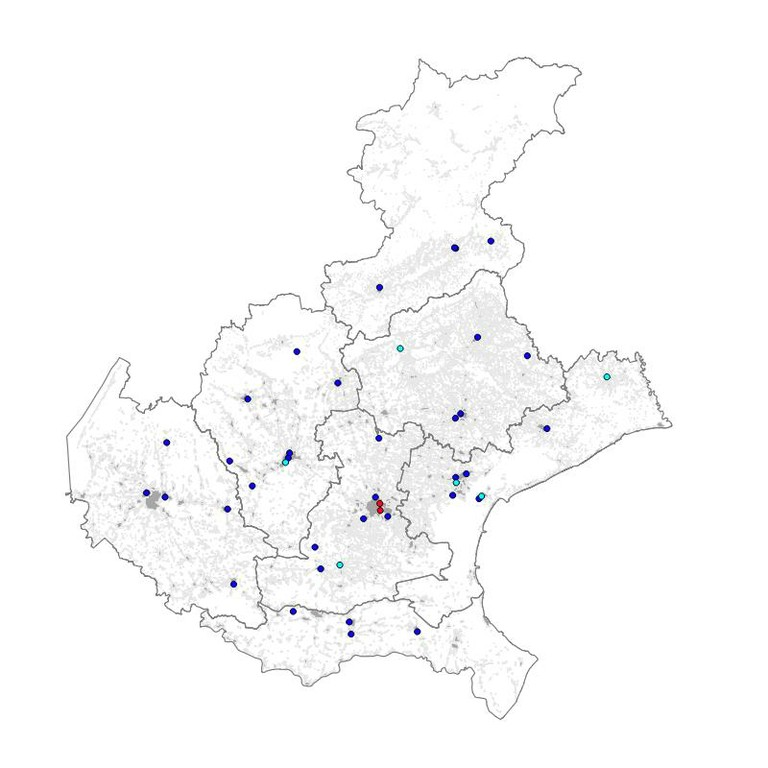
\includegraphics[width=0.7\textwidth]{images/ARPAV stazioni rete 2019.jpg}
    \caption{ARPAV monitoring netowrk in the Veneto region, Italy\cite{arpav}}
    \label{fig:arpav-map}
\end{figure}
\subsection{Low-cost sensors}
The \gls{epa} also provides the Air Sensor Guidebook\cite{williams2014air} which gives extensive information on air quality and low-cost sensors. Due to their prohibitive cost and complexity, conventional air pollution monitoring systems have low spacial and temporal resolution. Low-cost sensors, instead, can be deployed more diffusely with high spacial and temporal resolution, while trading most of their accuracy. They are, in fact, heavily influenced by many factors, especially temperature, humidity, wind and presence of other gases in the air.  Due to their lightweight, only low-cost sensors can be mounted on drones: the aforementioned influence factors could introduce even more inaccuracy, especially wind generated from the rotors.
\cite{s151229859} among other things presents an evaluation of air quality sensors classifying their performances by the most important parameters.
\subsection{Drone systems}
Coordinating data collection and movements is quite hard, considering the low computational power of UAVs, the inaccuracy of GPS and the general wireless communication issues. Ref [5] is a survey on the communication issues releted to drone networks. The energy constraint is really impactful on long missions and poses a major limitation to the spreading of drone technology. Drones have excellent mobility and data gathering prowess, but cannot always rely on coming back to the base to deliver their information. Implementing reasonable communication protocols and algorithms is necessary to improve efficiency. 
\subsection{Drone monitoring and sensing}
Thanks to their mobility and flying movement, drone monitoring and sensing capabiliteis are very valuable. In urban settings \gls{uavs} can monitor noise, traffic, light, wind, temperature, humidity, air quality and many other parameters.
As shown earlire, conventional air quality monitoring systems have very low spatial and temporal resolution. \gls{uavs} based systems could measure specific areas with great convenience and felxibility and hybrid ground and air based solutions could routinely track the air pollution levels of parts of a city. \cite{7946542}, \cite{evangelatos2015airborne}, \cite{8675167}, \cite{8662050} propose different solutions for a \gls{wsn} using \gls{uavs}. \cite{8675167} in particular examines an application in smart cities, where a hybrid ground and air based system tracks an urban area.
\section{Dissertation structure}
This dissertation describes the \gls{aria} project solution for the monitoring of air pollution. It is divided into 6 chapters:
\begin{itemize}
    \item Chapter 1 describes the introduction, an overview on the topic of air pollution, the motivation to approach the problem, the motivation of the proposed solution, related works, the state of the art and the dissertation objective.
    \item Chapter 2 describes the system architecture, that is the \gls{uavs} that are being used, their design, specifications and functionality.
    \item Chapter 3 describes the sensor payload, the motivation of the adopted sensors and their use.
    \item Chapter 4 describes the software implementation for the data collection of the sensors and the communication of the \gls{uavs}.
    \item Chapter 5 shows the results of a test flight using the proposed solution.
    \item Chapter 6 presents what conclusions can be taken after all the developed work, and what improvements can be done in the future.
\end{itemize}
\section{Dissertation objective}
The objective of this dissertation is to describe the solution proposed by the \gls{aria} project for air pollution monitoring, in particular the software impelementation, to show preliminary results and discuss their revelance in future applications.
    \clearpage
    \chapter{ARIA project}
\section{Overview}
ARIA project was created by a group of students from the Department of Industrial Engineering, University of Padova, under the suggestion and guidance of personnel staff of the Center for Space Studies and Activities (CISAS) of the same University. The core motivation that brought together these students was the desire of researching new fields of application for drone technology. ARIA project’s scenario is investigation about drones usage within air quality monitoring. Environmental pollution is becoming every day more threatening for our health and we wanted to develop a tool to monitor it in 3D. the project is funded by the Department of Industrial Engineering of our University.
\section{Proposal presentation}
ARIA project’s ultimate goal is gathering data about the
values of major pollutants in urban areas at various heights.
Our tool will be a vertical drone swarm equipped with low-cost sensors and deployable by utilizing GPS coordinates. The
information will be stored in a database, so that they can be
post-processed and published whenever appropriate. The most
interesting activity could be creating a contemporary vertical
profile of pollutants concentrations for various time-periods.
We’ve chosen to work with UAVs because after reading
literature about environmental monitoring, we found omissions
in Wireless Sensor Networks. The use of this new technology
was already recommended thanks to its speed, mobility and
capability to fly at different heights. The main constraint was
the unavailability of low-cost and low bulk drones.
To differentiate ourselves from previous studies (since our
knowledge would not be able to compete with them anyway)
we wanted to explore vertical swarms. The study of pollution
at different heights is not a popular topic and we wanted to
investigate it.
The task for the multicopter will have a standard implementation: usually it will be a simple request to move towards some
GPS coordinates, hover there while collecting samples and then
return to the base whenever the time is up or the battery is too
low, or move through different GPS waypoints, hovering at each one to allow the sensors to adjust and collect the data. 
The gas sensors have a response time of around 30s which needs to be taken into consideration.
The flight will be planned before departure from a
terminal. The vertical deployment doesn’t need to be extremely
precise, since sensor’s accuracy is not sufficient for slight
misplacements to matter, and  . Since our approach will be careful
and gradual, each entity belonging to the swarm will not
communicate with the others. Considering this fact, we know
the term ”swarm” is being used inappropriately. Wireless
communication and real swarm implementation will follow as
the project unfolds.


    \clearpage
    \chapter{ARIA: System architecture}

    \clearpage
    \chapter{Sensor Payload}
    \clearpage
    \chapter{ARIA: Software implementation}
    \clearpage
    \chapter{ARIA: Field Test}
A field test was performed in a trafficked area in Padova (Italy) in autumn 2021 (see Figure \ref{fig:3d-map}), mainly to test the sensors. The drones were carried by hand. the Figures below contain the data collected by the two drones, the mission times are synchronized and the Arduino drone also has the data for the NO sensor.


therefore data was collected at ground level except for the portion between xxx and xxx seconds when we set the drone on the bridge above the road at xxx m.

\begin{figure}[h!]
    \centering
    \begin{subfigure}[b]{0.45\textwidth}
        \centering
        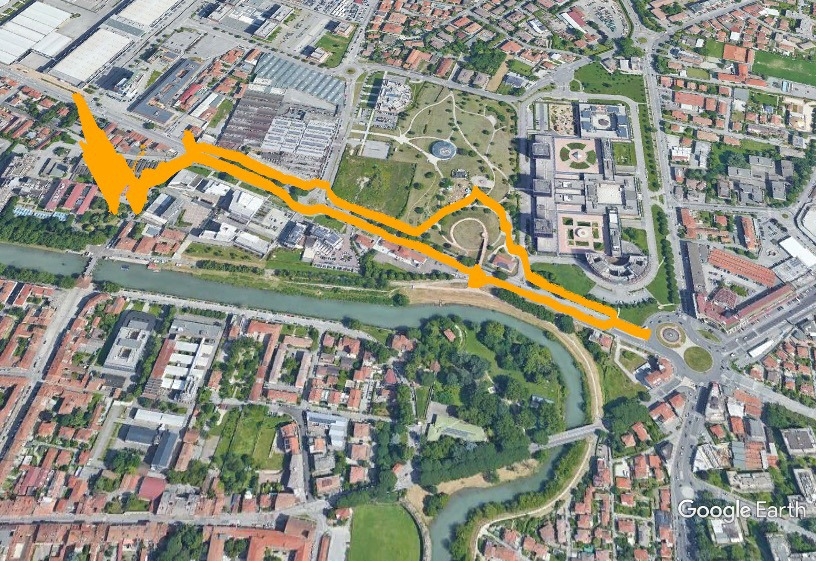
\includegraphics[width=\textwidth]{images/flight-data/3d-map.jpg}
        \caption{}
        \label{fig:3d-map}
    \end{subfigure}
    \hfill
    \begin{subfigure}[b]{0.45\textwidth}
        \centering
        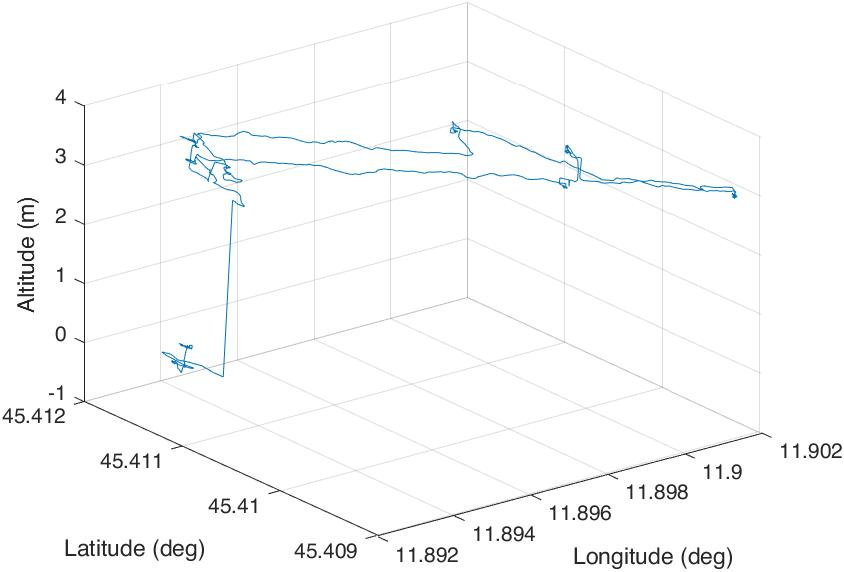
\includegraphics[width=\textwidth]{images/flight-data/raspberry/ALT_3D_R.jpg}
        \caption{}
        \label{fig:testflight-alt}
    \end{subfigure}
       \caption{3D map and 3D altitude plot}
       \label{fig:testflight-telemetry}
\end{figure}

\begin{figure}
    \centering
    \begin{subfigure}[b]{0.45\textwidth}
        \centering
        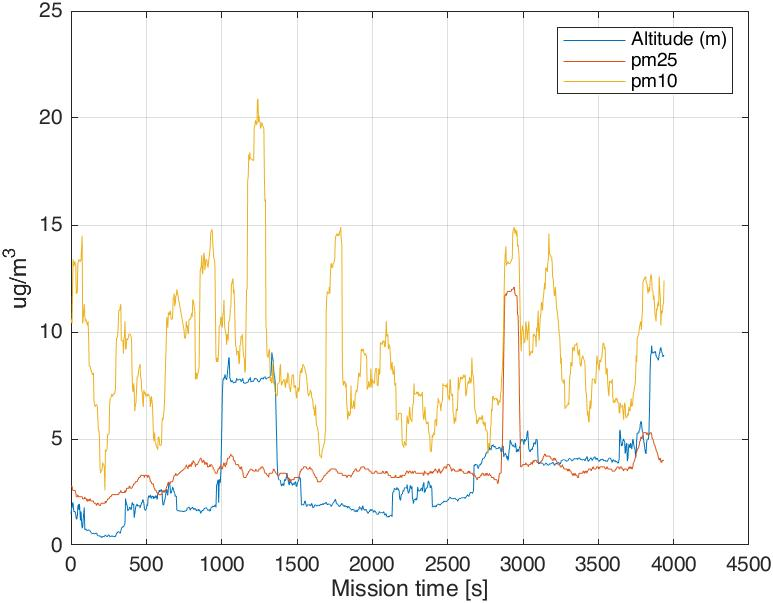
\includegraphics[width=\textwidth]{images/flight-data/raspberry/pms_R.jpg}
        \caption{Raspberry Pi drone PM sensor data}
        \label{fig:pms_R}
    \end{subfigure}
    \hfill
    \begin{subfigure}[b]{0.45\textwidth}
        \centering
        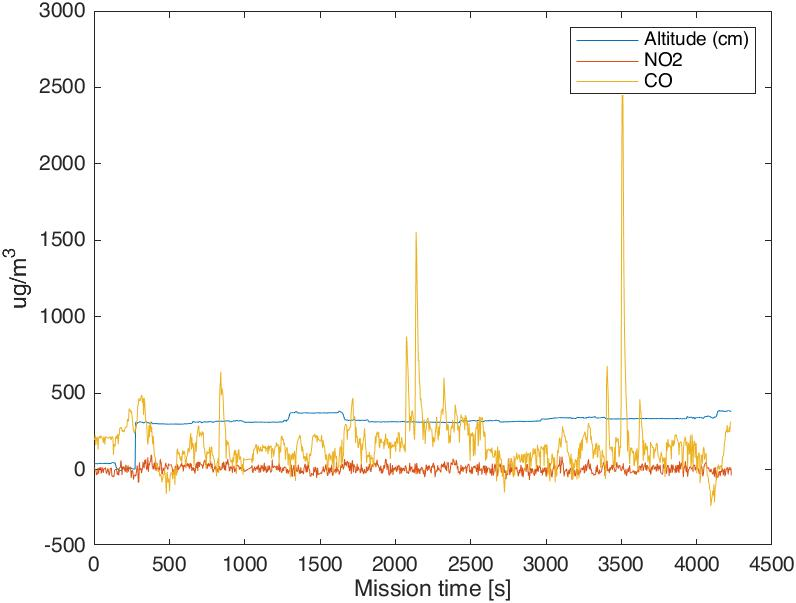
\includegraphics[width=\textwidth]{images/flight-data/raspberry/ariasensors_R.jpg}
        \caption{Raspberry Pi drone gas sensor data}
        \label{fig:ariasensors_R}
    \end{subfigure}

    \centering
    \begin{subfigure}[b]{0.45\textwidth}
        \centering
        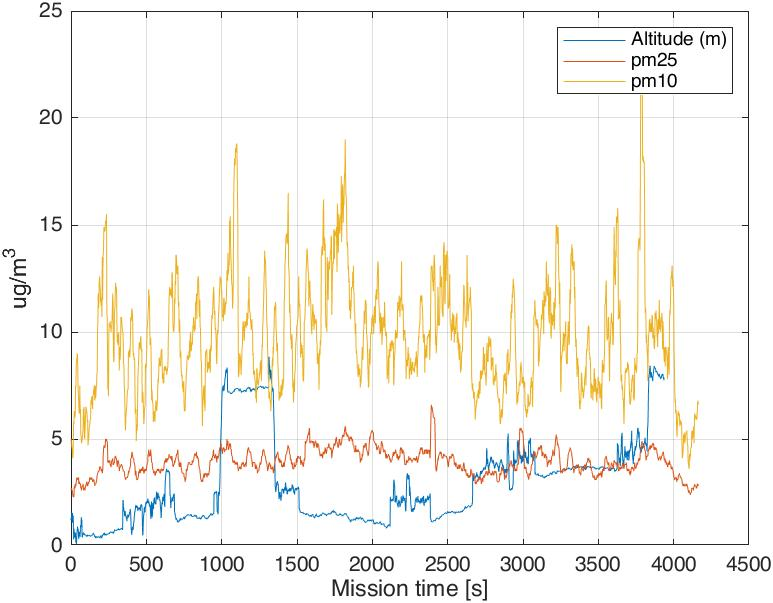
\includegraphics[width=\textwidth]{images/flight-data/arduino/pms.jpg}
        \caption{Arduino drone PM sensor data}
        \label{fig:pms}
    \end{subfigure}
    \hfill
    \begin{subfigure}[b]{0.45\textwidth}
        \centering
        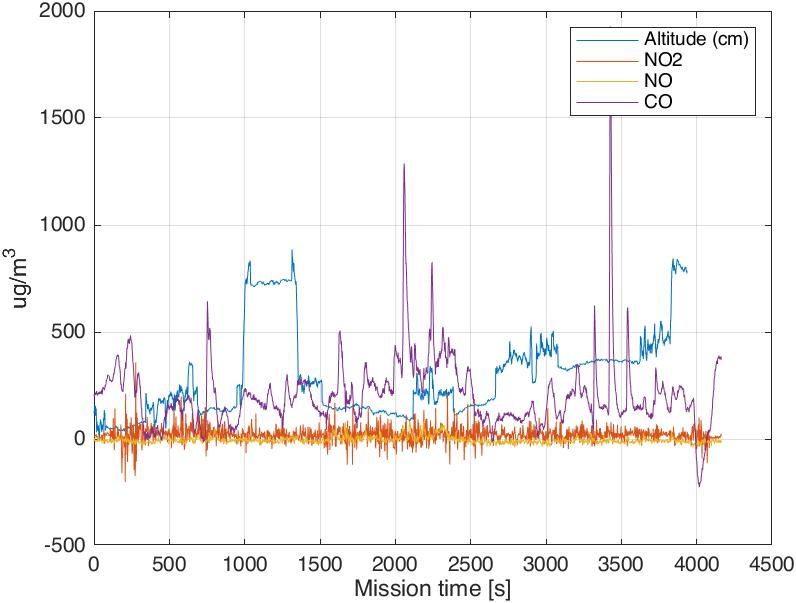
\includegraphics[width=\textwidth]{images/flight-data/arduino/ariasensors.jpg}
        \caption{Arduino drone gas sensor data}
        \label{fig:ariasensors}
    \end{subfigure}
    \hfill
       \caption{PM and gas sensors data from the Raspberry Pi drone (top two) and the Arduino drone (bottom two)}
       \label{fig:pms-and-sensors}
\end{figure}

\begin{figure}
    \centering
    \begin{subfigure}[b]{0.45\textwidth}
        \centering
        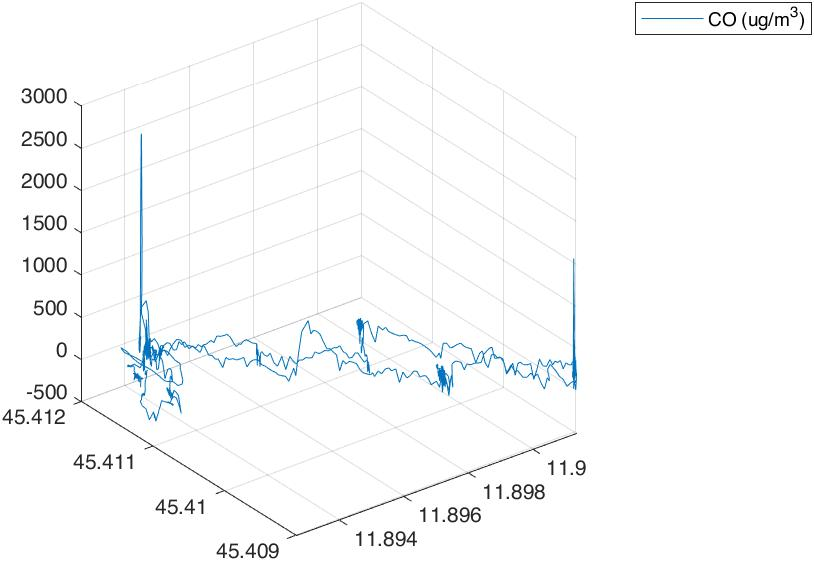
\includegraphics[width=\textwidth]{images/flight-data/raspberry/CO_3D_R.jpg}
        \caption{Raspberry Pi $CO$}
        \label{fig:CO_3D_R}
    \end{subfigure}
    \hfill
    \begin{subfigure}[b]{0.45\textwidth}
        \centering
        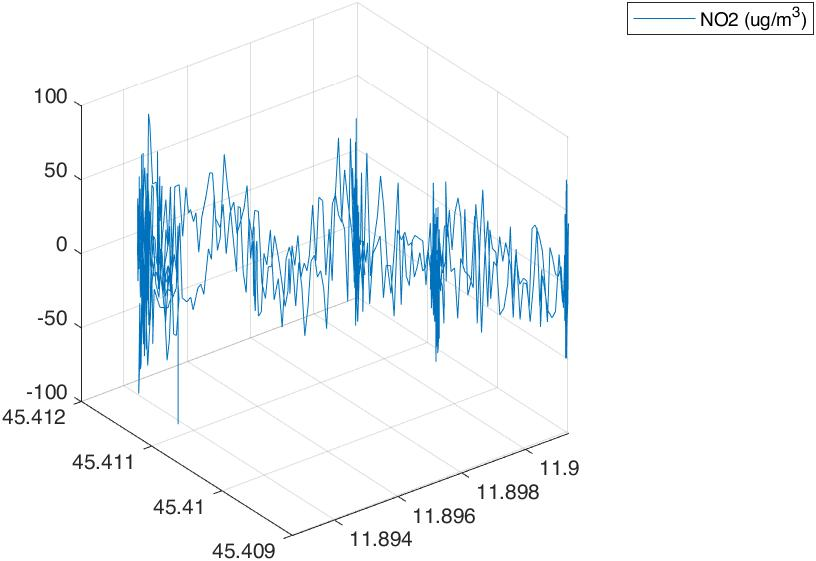
\includegraphics[width=\textwidth]{images/flight-data/raspberry/NO2_3D_R.jpg}
        \caption{Raspberry Pi $NO_2$}
        \label{fig:NO2_3D_R}
    \end{subfigure}

    \centering
    \begin{subfigure}[b]{0.45\textwidth}
        \centering
        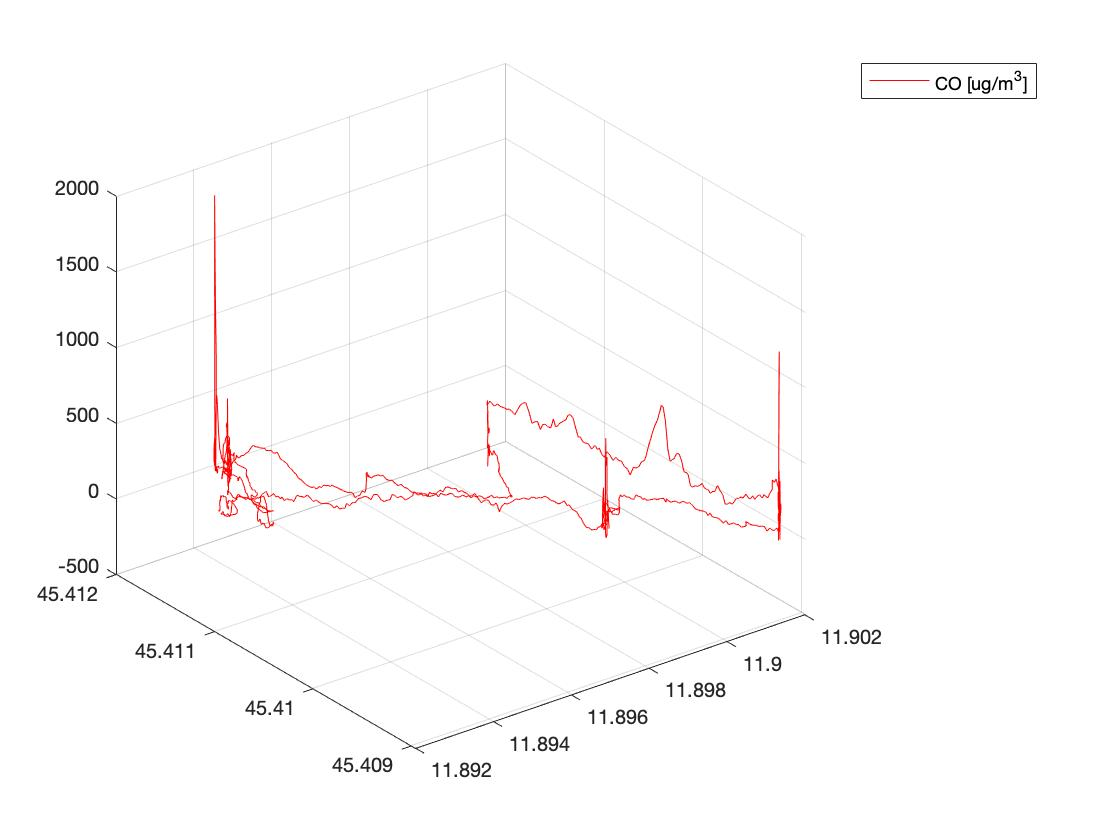
\includegraphics[width=\textwidth]{images/flight-data/arduino/CO_3D.jpg}
        \caption{Arduino $CO$}
        \label{fig:CO_3D}
    \end{subfigure}
    \hfill
    \begin{subfigure}[b]{0.45\textwidth}
        \centering
        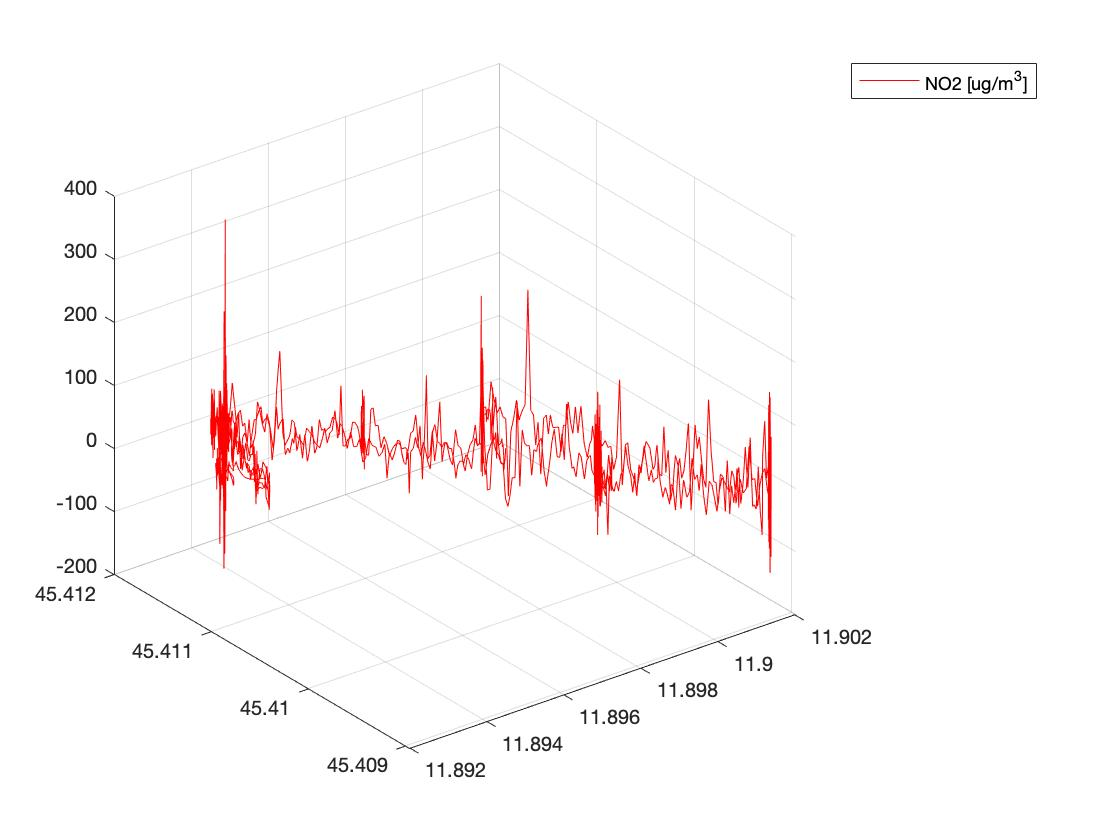
\includegraphics[width=\textwidth]{images/flight-data/arduino/NO2_3D.jpg}
        \caption{Arduino $NO_2$}
        \label{fig:NO2_3D}
    \end{subfigure}
    
    \begin{subfigure}[b]{0.45\textwidth}
        \centering
        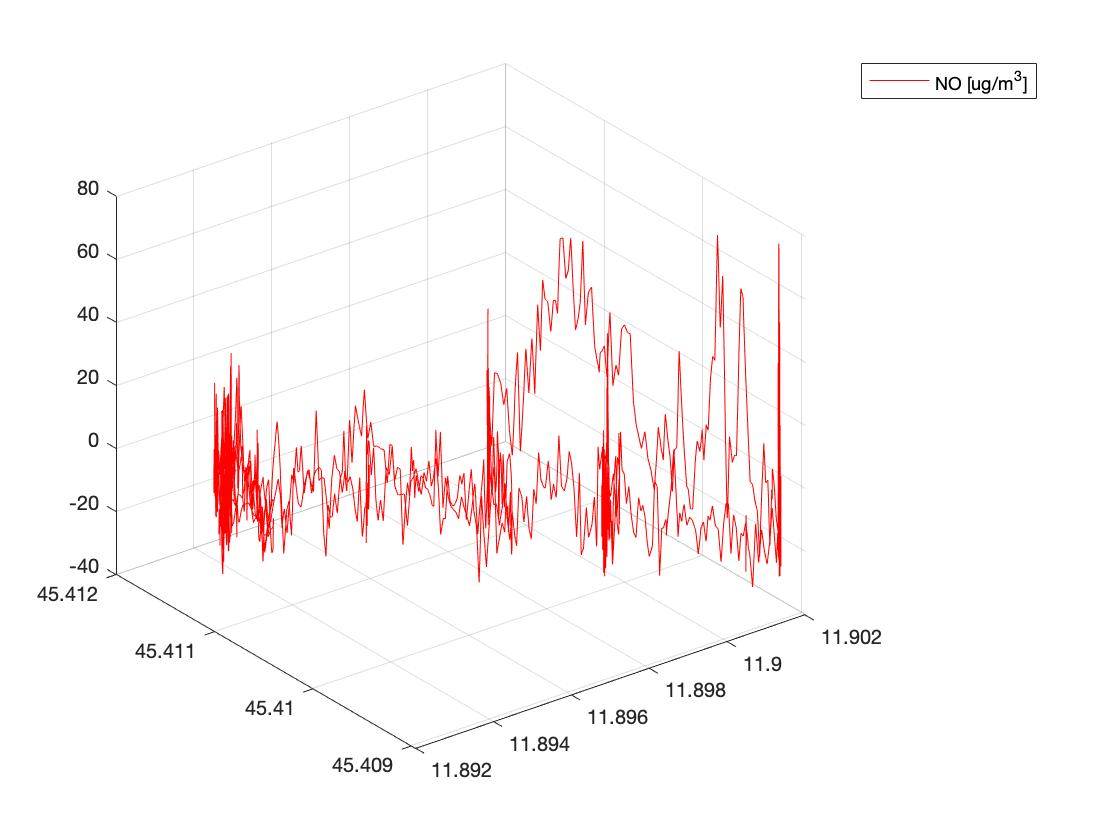
\includegraphics[width=\textwidth]{images/flight-data/arduino/NO_3D.jpg}
        \caption{Arduino $NO$}
        \label{fig:NO_3D}
    \end{subfigure}
       \caption{3D plots of the gas sensors data, Raspberry Pi drone data is in blue (top two), Arduino drone data is in red (bottom three)}
       \label{fig:3Ds}
\end{figure}
    \clearpage
    \chapter{Conclusions and future work}
    \clearpage
    \printbibliography[
        heading=bibintoc,
        title={Bibliography}
    ]
\end{document}